\documentclass[journal,twocolumn]{IEEEtran}
\usepackage[utf8]{inputenc}
\usepackage[spanish]{babel}
\usepackage{graphicx}
\usepackage{amsmath}
\usepackage{amsfonts}
\usepackage{amssymb}
\usepackage[hidelinks]{hyperref}
\usepackage{geometry}
\usepackage{cite}
% \usepackage{float}  % removido para evitar conflictos de identificadores con IEEEtran
\usepackage{listings}
\usepackage{xcolor}
\usepackage{booktabs}
\usepackage{tikz}
\usetikzlibrary{shapes,arrows,positioning,calc,babel,fit,decorations.pathreplacing}
\usepackage{placeins}


\pgfdeclarelayer{background}
\pgfsetlayers{background,main}

% Configuración de página
\geometry{a4paper, margin=1.8cm}

% Configuración de código
\lstset{
    language=Python,
    basicstyle=\ttfamily\scriptsize,
    keywordstyle=\color{blue},
    stringstyle=\color{red},
    commentstyle=\color{green!60!black},
    breaklines=true,
    showstringspaces=false,
    frame=single
}

\title{Implementación de un Sistema de Control de Lazo Cerrado para la Estabilización Térmica de un Centro de Datos mediante Control Proporcional-Integral-Derivativo (PID)}

\author{
    \IEEEauthorblockN{Matias Ezequiel Pormi} \\
    \IEEEauthorblockA{Facultad Regional Buenos Aires, Universidad Tecnológica Nacional \\
    Comisión: K-4011 \\
    Profesor: Ing. Omar Oscár Civale \\
    Fecha: Julio de 2026}
}

\begin{document}

\maketitle

\begin{abstract}
En el presente trabajo se desarrolla el diseño, modelado y validación de un sistema de control automático en lazo cerrado para la regulación de temperatura en el pasillo frío de un centro de datos. Se emplea un modelo de primer orden con tiempo muerto (FOPTD) para caracterizar la dinámica térmica de la planta, utilizando parámetros obtenidos de investigaciones experimentales recientes. El controlador implementado es de tipo PID paralelo, sintonizado para garantizar una respuesta temporal estable y amortiguada ante retardos de transporte. La validación se realiza mediante simulación computacional, analizando la respuesta ante escalones de referencia y la capacidad de rechazo de perturbaciones críticas como ataques de denegación de servicio (DoS) térmicos. Los resultados confirman la eficacia de la acción integral para eliminar el error en estado estable y la capacidad del sistema para mantener condiciones ambientales óptimas según estándares ASHRAE.
\end{abstract}

\begin{IEEEkeywords}
Control PID, Data Center, Tiempo Muerto, Aproximación de Padé, Estabilidad del Sistema, Simulación en Python.
\end{IEEEkeywords}

\tableofcontents
\vspace{1em}

\section{Introducción}
La infraestructura crítica de centros de datos requiere un control ambiental extremadamente riguroso debido a la alta sensibilidad térmica de los componentes semiconductores modernos. En entornos de alta densidad, como los clústeres de computación en la nube, la generación de calor es una variable volátil que depende directamente de la carga de procesamiento del servidor. Un incremento descontrolado en la temperatura no solo compromete la vida útil del hardware (acelerando fallos por electromigración y fatiga térmica), sino que también degrada significativamente la eficiencia energética del centro de datos (medida a través del \textit{Power Usage Effectiveness}, PUE).

El objetivo de este proyecto es diseñar un lazo de control cerrado que regule la temperatura de inyección de aire frío mediante la modulación de ventiladores de velocidad variable en una unidad de acondicionamiento de aire de precisión (CRAC). Se busca un comportamiento dinámico que equilibre la velocidad de respuesta con la estabilidad robusta, garantizando que el sistema pueda absorber picos térmicos severos sin entrar en oscilaciones divergentes.

\section{Alcance y Estructura del Sistema}
\label{sec:alcance}

\subsection{Contexto y Segmento de Mercado}
El sistema se enmarca en el mercado de la climatización de precisión para centros de datos corporativos y de proveedores Cloud. Se utiliza la técnica de confinamiento de pasillo frío, donde el aire a baja temperatura es inyectado desde el suelo técnico y aspirado por la parte frontal de los racks de servidores. La separación física de los flujos de aire frío y caliente (pasillo caliente) es esencial para evitar la mezcla termodinámica y optimizar la ganancia térmica de la planta. Como referencia de hardware de precisión, se consideran las unidades de la línea \textbf{Schneider Electric Uniflair™} (Serie LE/DX).

\begin{figure}[htbp]
    \centering
    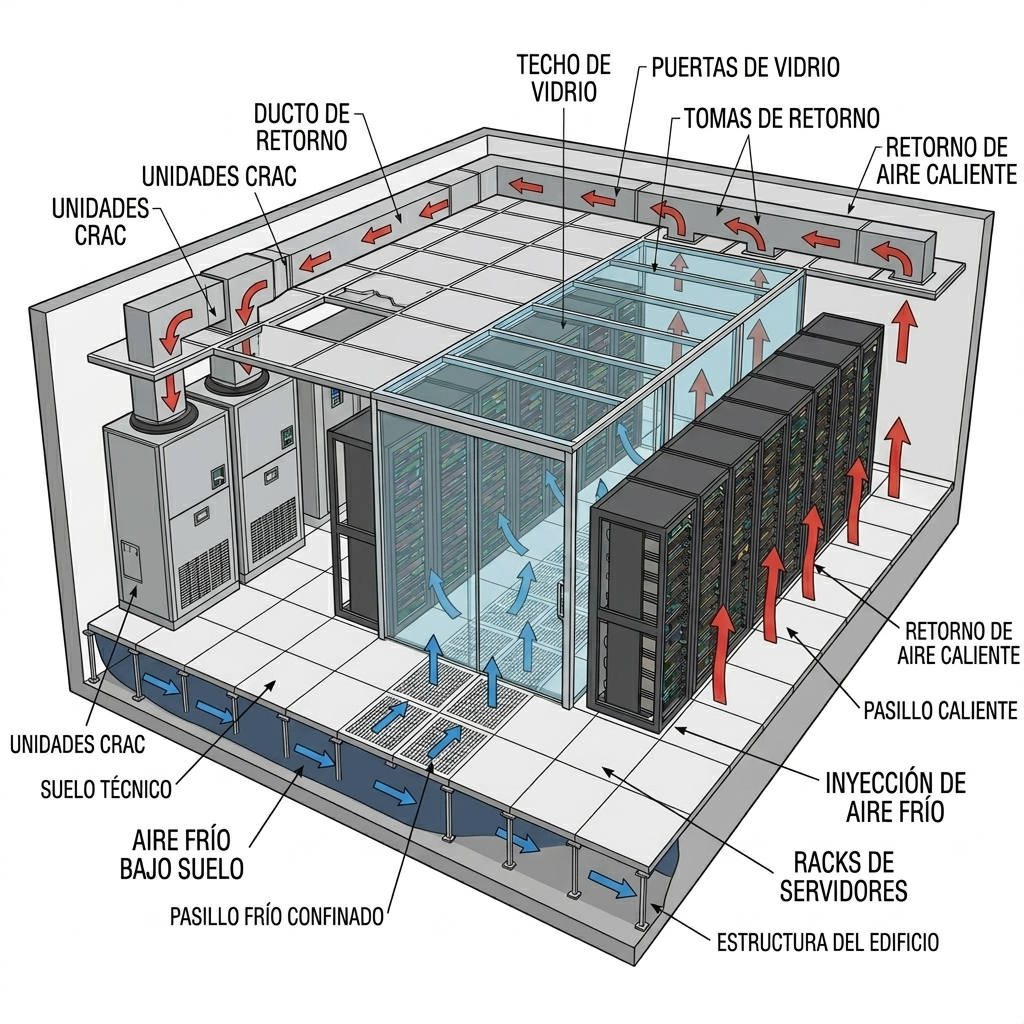
\includegraphics[width=\linewidth]{esquema_pasillo_frio.jpg}
    \caption{Esquema de confinamiento de pasillo frío y dinámica de flujo de aire en el Data Center. Se observa la inyección de aire frío por el suelo técnico elevado (raised floor), la aspiración por los servidores, y el retorno de aire caliente (hot air return) hacia la unidad CRAC/CRAH.}
    \label{fig:pasillo_frio}
\end{figure}

\subsection{Carga del Sistema}
La carga térmica a disipar está constituida por la \textbf{Carga Térmica de IT} ($Q_{IT}$), generada por los racks de servidores de computación activa. Esta carga se modela en kilowatts [kW] y es una variable dinámica que fluctúa según el procesamiento de transacciones. Ante un pico súbito de tráfico, la disipación térmica del silicio actúa de forma inmediata, elevando la temperatura del flujo de aire adyencente.

\subsection{Puntos de Interconexión con el Exterior}
\begin{itemize}
    \item \textbf{Consigna de Operación (Setpoint):} Temperatura de consigna de inyección definida por el operador según las guías ASHRAE TC 9.9, típicamente a $22^\circ$C (rango permitido de $18^\circ$C a $27^\circ$C).
    \item \textbf{Suministro Energético:} Interfaz con la red eléctrica trifásica industrial (380V/480V, 50/60 Hz) para alimentar los motores de conmutación electrónica (EC) de los sopladores y la etapa del compresor.
    \item \textbf{Gestión de Datos:} Protocolos de comunicación industrial (Modbus TCP/IP o SNMP) para la comunicación del controlador con el sistema de monitoreo DCIM (\textit{Data Center Infrastructure Management}).
    \item \textbf{Interfaces Físicas de Aire:} Acoplamiento fluidodinámico entre la descarga del evaporador de la CRAC y la cara frontal del rack (pasillo frío), y el retorno del pasillo caliente.
\end{itemize}

\subsection{Transductores y Elementos de Medición}
El elemento de realimentación principal es un \textbf{sensor de temperatura industrial de resistencia de platino (RTD Pt100)} de alta precisión acoplado a un transmisor electrónico linealizado. El transmisor compensa la pequeña no linealidad natural de la resistencia del platino y convierte la medición de temperatura en una señal analógica de tensión ($0$-$10$\,V DC) de forma perfectamente lineal dentro del rango de operación industrial de la planta ($0^\circ$C a $50^\circ$C).

La ecuación del transductor lineal se expresa como:
\begin{equation}
    V_{sensor}(T) = V_{min} + \left( \frac{V_{max} - V_{min}}{T_{max} - T_{min}} \right) (T - T_{min})
\end{equation}
Sustituyendo los límites del rango configurado ($T_{min} = 0^\circ$C, $T_{max} = 50^\circ$C, $V_{min} = 0$\,V, $V_{max} = 10$\,V), se obtiene la relación directa:
\begin{equation}
    V_{sensor}(T) = 0.2 \cdot T
\end{equation}
donde $T$ es la temperatura en $^\circ$C y $V_{sensor}(T)$ es la tensión analógica entregada al controlador. Bajo esta relación, el Setpoint nominal de $22^\circ$C se corresponde con $4.4$\,V y la temperatura inicial de $28^\circ$C equivale a $5.6$\,V. Posteriormente, esta tensión es digitalizada por un Convertidor Analógico-Digital (ADC) de 10 bits ($0$-$1023$ unidades de cuantización, correspondientes a $0$-$10$\,V).

\subsection{Actuadores y Elementos de Acción}
\begin{itemize}
    \item \textbf{Ventiladores EC (Electronically Commutated):} Ventiladores radiales de alta eficiencia movidos por motores de imanes permanentes con electrónica integrada. Reciben una señal analógica de control de $0$-$10$\,V DC del controlador y varían su caudal de aire de forma proporcional del 0\% al 100\% de su capacidad nominal.
    \item \textbf{Válvula de Expansión Electrónica (EEV):} Modula el caudal másico de refrigerante en el lazo de expansión directa de la CRAC para ajustar la potencia frigorífica neta entregada al serpentín.
\end{itemize}

A los fines del modelado y para simplificar el desarrollo analítico, la dinámica de los actuadores se considera ideal: su respuesta es instantánea frente a la constante de tiempo térmica de la sala ($\tau = 35$\,s). En consecuencia, en el diagrama de bloques de la Fig.~\ref{fig:bloques} se modelan con una ganancia unitaria $G_a(s) = 1$, de modo que $U(s) = U_{PID}(s)$.

\subsection{Variables, Unidades y Rangos}
\begin{itemize}
    \item \textbf{Variable Controlada ($y(t)$):} Temperatura de suministro en pasillo frío [$^\circ$C]. Rango típico de operación: $15^\circ$C a $30^\circ$C.
    \item \textbf{Referencia ($r(t)$):} Consigna de temperatura o Setpoint [$^\circ$C]. Rango recomendado por ASHRAE: $18^\circ$C a $27^\circ$C.
    \item \textbf{Variable Manipulada ($u(t)$):} Esfuerzo de enfriamiento o potencia de enfriamiento [\%] ($0$-$100$\%).
    \item \textbf{Perturbación ($d(t)$):} Carga térmica IT extra inyectada en el pasillo caliente o pérdidas térmicas por apertura de puertas [$^\circ$C].
\end{itemize}

\subsection{Amplificador de Error y Señales de Error/Realimentación}
El comparador (punto suma) resta la señal de realimentación medida $y_f(t)$ de la referencia $r(t)$. La señal de error resultante es $e(t) = r(t) - y_f(t)$. Debido a que la planta tiene una ganancia estática negativa (un aumento en la potencia de enfriamiento $u(t)$ disminuye la temperatura $y(t)$), el lazo cerrado de control digital calcula la acción del controlador invirtiendo este error o aplicando ganancias de sintonía negativas para mantener el lazo estable con realimentación negativa constructiva. El amplificador de error se implementa en software dentro del procesador digital de la CRAC.

\subsection{Relación entre Señales Analógicas y Digitales}
El lazo físico es analógico y continuo, pero el algoritmo PID se ejecuta digitalmente en un microcontrolador o PLC de precisión. Esto requiere:
\begin{enumerate}
    \item \textbf{Discretización de Señales:} Un ADC lee la tensión del transmisor del sensor Pt100 con un tiempo de muestreo de $T_s = 100$\,ms. Dado que la constante de tiempo térmica de la sala ($\tau = 35$\,s) es mucho mayor que $T_s$ ($\tau \gg T_s$), la aproximación por modelado continuo en Laplace es plenamente válida.
    \item \textbf{Conversión DAC:} La salida de control digital (0-100\%) es convertida en una señal física de $0$-$10$\,V mediante salidas analógicas con modulación por ancho de pulsos (PWM) filtradas con una resolución de 8 bits.
    \item \textbf{Conversión de Unidades en Software y Compensación de $H(s)$:} Para posibilitar que las variables internas y de consigna se operen directamente en grados Celsius ($^\circ$C), el firmware del controlador realiza la conversión de la lectura del sensor dividiendo el valor digital por la ganancia del transductor ($H(s) = 0.2$\,V/$^\circ$C). Esta operación de calibración en software compensa la ganancia del sensor, resultando en una realimentación efectiva unitaria ($H_{eff}(s) = 1$). Por lo tanto, las constantes de sintonización propuestas ($K_p = 2.5$, $K_i = 0.08$, $K_d = 0.5$) son ganancias del controlador de software. Físicamente, para mantener el mismo comportamiento dinámico en el lazo analógico (dominio de tensión de $0$-$10$\,V), las ganancias físicas equivalentes en tensión son 5 veces mayores ($K_{p,phys} = 12.5$\,\%/V, $K_{i,phys} = 0.4$\,\%/(V$\cdot$s), $K_{d,phys} = 2.5$\,\%$\cdot$s/V).
\end{enumerate}

\subsection{Diagrama de Bloques}
La estructura del sistema sigue la topología de realimentación unitaria con adición de perturbación. En la Fig. \ref{fig:bloques} se detalla la interconexión.

\begin{figure*}[!t]
    \centering
    \shorthandoff{<}
    \shorthandoff{>}
    \resizebox{\textwidth}{!}{%
    \begin{tikzpicture}[auto, >=stealth, scale=0.85, transform shape]
        % Style definitions
        \tikzset{
            block/.style={draw, fill=white, rectangle, minimum height=2.8em, minimum width=7.5em, align=center, line width=0.6pt, rounded corners=1pt, font=\small},
            sum/.style={draw, fill=white, circle, minimum size=1.5em, align=center, line width=0.6pt},
            input/.style={coordinate},
            output/.style={coordinate}
        }

        % Nodes
        \node [input] (input) {};
        
        % Transmitter
        \node [block, right=1.0cm of input] (transmitter) {$H_r(s) = 0.2$\,V/$^\circ$C};
        
        % Error Summing Junction
        \node [sum, right=1.0cm of transmitter] (sum1) {};
        
        % Split point for PID (defined as coordinate along the line)
        \coordinate (split) at ($(sum1.east) + (1.2,0)$);
        \coordinate (split_box) at ($(sum1.east) + (0.9,0)$);
        
        % Parallel PID blocks - placed relative to sum1
        \node [block, right=2.0cm of sum1] (i) {I \\ $\frac{K_i}{s}$};
        \node [block, above=0.6cm of i] (p) {P \\ $K_p$};
        \node [block, below=0.6cm of i] (d) {D \\ $K_d \cdot s$};
        
        % PID Summing Junction
        \node [sum, right=1.2cm of i] (sum_pid) {};
        
        % Actuator (unity gain for simplicity)
        \node [block, right=0.8cm of sum_pid] (actuator) {Actuador \\ $G_a(s) = 1$};
        
        % Thermal Plant
        \node [block, right=0.8cm of actuator] (plant) {Planta \\ $G_p(s)$};
        
        % Disturbance Summing Junction
        \node [sum, right=0.8cm of plant] (sum2) {};
        
        % Output
        \node [output, right=0.8cm of sum2] (output) {};
        
        % Disturbance Input
        \node [align=center, above=0.8cm of sum2, font=\small] (dist) {Perturbación \\ $D(s)$};
        
        % Sensor (placed below the controller, aligned with i)
        \node [block, below=2.0cm of i] (sensor) {Sensor Pt100 \\ $H(s) = 0.2$};
        
        % Connections
        % Input to Transmitter
        \draw [->, line width=0.6pt] (input) -- (transmitter);
        \node [align=left, left=0.15cm of input, font=\small] {Consigna \\ $R(s)$\,[$^\circ$C]};
        
        % Transmitter to Sum1
        \draw [->, line width=0.6pt] (transmitter) -- node [above] {$V_{sp}(s)$} (sum1);
        \node at ($(sum1.center) + (-4pt, 4pt)$) {\scriptsize $+$};
        
        % Sum1 to Split and Middle Block (I)
        \draw [line width=0.6pt] (sum1) -- node [above, pos=0.45] {$E(s)$} (split);
        \draw [->, line width=0.6pt] (split) -- (i.west);
        
        % Split to P and D
        \draw [->, line width=0.6pt] (split) |- (p.west);
        \draw [->, line width=0.6pt] (split) |- (d.west);
        
        % P, I, D to Sum PID
        \draw [->, line width=0.6pt] (p.east) -| (sum_pid.north);
        \node at ($(sum_pid.center) + (-4pt, 4pt)$) {\scriptsize $+$};
        
        \draw [->, line width=0.6pt] (i.east) -- (sum_pid.west);
        \node at ($(sum_pid.center) + (-4pt, -3pt)$) {\scriptsize $+$};
        
        \draw [->, line width=0.6pt] (d.east) -| (sum_pid.south);
        \node at ($(sum_pid.center) + (3pt, -4pt)$) {\scriptsize $+$};
        
        % Sum PID to Actuator
        \draw [->, line width=0.6pt] (sum_pid) -- node [above] {$U_{PID}(s)$} (actuator);
        
        % Actuator to Plant
        \draw [->, line width=0.6pt] (actuator) -- node [above] {$U(s)$} (plant);
        
        % Plant to Sum2
        \draw [->, line width=0.6pt] (plant) -- (sum2);
        \node at ($(sum2.center) + (-4pt, 4pt)$) {\scriptsize $+$};
        
        % Sum2 to Output
        \draw [->, line width=0.6pt] (sum2) -- (output);
        \node [align=left, right=0.15cm of output, font=\small] {Temperatura \\ $Y(s) \equiv T(s)$\,[$^\circ$C]};
        
        % Disturbance to Sum2
        \draw [->, line width=0.6pt] (dist) -- (sum2);
        \node at ($(sum2.center) + (4pt, 4pt)$) {\scriptsize $+$};
        
        % Feedback Path
        \coordinate (feedback) at ($(sum2.east) + (0.4,0)$);
        \draw [->, line width=0.6pt] (feedback) |- (sensor.east);
        \draw [->, line width=0.6pt] (sensor.west) -| node [above, pos=0.25, font=\small] {$V_{sensor}(s)$} (sum1.south);
        \node at ($(sum1.center) + (-4pt, -4pt)$) {\scriptsize $-$};
        
        % Background Layer for Dashed Box
        \begin{pgfonlayer}{background}
            \node [draw, dashed, fill=gray!10, fit=(split_box) (p) (i) (d) (sum_pid), inner sep=0.18cm] (Gc) {};
            \node [above right, font=\small] at (Gc.north west) {$G_c(s)$};
        \end{pgfonlayer}
    \end{tikzpicture}%
    }
    \shorthandon{<}
    \shorthandon{>}
    \caption{Diagrama de bloques del lazo de control de temperatura del Data Center. Se detalla la señal de referencia $R(s)$, el transmisor de referencia $H_r(s)$, el error $E(s)$, el controlador PID $G_c(s)$, el actuador con ganancia unitaria $G_a(s) = 1$, la planta térmica $G_p(s)$, la perturbación $D(s)$ y el sensor de realimentación $H(s)$.}
    \label{fig:bloques}
\end{figure*}

\section{Modelado Matemático}
\label{sec:modelado}

\subsection{Identificación de la Planta ($G_p$)}
Para obtener la dinámica de la planta, se emplea la metodología de \textbf{Identificación por Respuesta al Escalón}. Se induce una variación escalón en el esfuerzo de los ventiladores de la CRAC y se registra el transitorio de la temperatura. Con base en el estudio experimental de \href{https://doi.org/10.3390/buildings16091752}{Liu et al. (2026)} \cite{liu2026}, el proceso se modela como un sistema de \textbf{Primer Orden con Tiempo Muerto (FOPTD)}:
\begin{equation}
    G_p(s) = \frac{K e^{-\theta s}}{\tau s + 1} = \frac{-0.25 e^{-4.5 s}}{35 s + 1}
\end{equation}
donde:
\begin{itemize}
    \item $K = -0.25\,^\circ$C/\% representa la ganancia estática del proceso. El signo negativo indica físicamente una relación inversa o de acción inversa (\textit{reverse-acting}): un incremento en la variable manipulada (esfuerzo o potencia de enfriamiento $u(t)$) produce una disminución en la variable controlada (temperatura del pasillo frío $y(t)$). Cuantitativamente, un aumento del 1\% en el esfuerzo de enfriamiento reduce la temperatura en $0.25\,^\circ$C en estado estacionario.
    \item $\tau = 35$\,s es la constante de tiempo térmica de la zona confinada (inercia térmica).
    \item $\theta = 4.5$\,s es el tiempo muerto o retardo de transporte, que modela el tiempo de tránsito del aire frío desde la descarga de la CRAC hasta el plano de los servidores.
\end{itemize}

\subsection{Aproximación de Padé}
El retardo de transporte $e^{-\theta s}$ representa un operador trascendente no racional. Para posibilitar el análisis dinámico en el dominio de Laplace, se aproxima mediante una expansión de Padé de segundo orden ($n=2$):
\begin{equation}
    e^{-\theta s} \approx \frac{\theta^2 s^2 - 6\theta s + 12}{\theta^2 s^2 + 6\theta s + 12}
\end{equation}
Sustituyendo $\theta = 4.5$\,s, la aproximación del retardo resulta en:
\begin{equation}
    e^{-4.5 s} \approx \frac{20.25 s^2 - 27 s + 12}{20.25 s^2 + 27 s + 12}
\end{equation}

\subsection{Controlador PID ($G_c$)}
El controlador utilizado sigue la ley analógica paralela clásica Proporcional-Integral-Derivativa:
\begin{equation}
    G_c(s) = K_p + \frac{K_i}{s} + K_d s
\end{equation}
\begin{itemize}
    \item \textbf{Acción Proporcional ($K_p$):} Proporciona la fuerza correctora proporcional a la desviación térmica actual, acelerando la respuesta del sistema.
    \item \textbf{Acción Integral ($K_i$):} Elimina el error remanente en estado estacionario ($e_{ss} = 0$) acumulando la historia del error, fundamental para absorber la carga térmica permanente de los servidores.
    \item \textbf{Acción Derivativa ($K_d$):} Introduce un efecto anticipativo y de amortiguamiento evaluando la derivada temporal del error, reduciendo el sobreimpulso provocado por la inercia y el retardo.
\end{itemize}

\section{Análisis de Estabilidad y Sintonización}

\subsection{Trayectoria Directa y Corrección de Signo}
Para analizar la estabilidad y diseñar la sintonía del controlador en lazo cerrado, es fundamental definir la estructura de las funciones de transferencia del sistema. En la teoría de control clásica, distinguimos dos conceptos clave:
\begin{enumerate}
    \item \textbf{Trayectoria Directa ($G_d(s)$):} Es la función de transferencia del camino de ida en el lazo, que va desde la señal de error en tensión $E(s)$ hasta la salida física del proceso $Y(s)$ (sin incluir el sensor de retorno). Físicamente, está compuesta por el controlador y la planta: $G_d(s) = G_c(s) G_p(s)$.
    \item \textbf{Lazo Abierto ($G_{ol}(s)$, del inglés \textit{open loop}):} Es la ganancia total recorrida al abrir el lazo cerrado justo antes del comparador de error. Se define formalmente como el producto de la trayectoria directa $G_d(s)$ y la función de transferencia del sensor en el camino de realimentación $H(s)$:
    \begin{equation}
        G_{ol}(s) = G_d(s) H(s) = G_c(s) G_p(s) H(s)
    \end{equation}
\end{enumerate}

Para ilustrar este concepto, la Fig.~\ref{fig:lazo_abierto} muestra el lazo de control abierto justo antes del comparador. Al inyectar una señal de prueba en ese punto y recorrer una vuelta completa —atravesando el controlador, la planta y el sensor— se obtiene la ganancia de lazo abierto $G_{ol}(s)$ como el producto de todas las transferencias del camino.

\begin{figure}[htbp]
    \centering
    \shorthandoff{<}
    \shorthandoff{>}
    \resizebox{\columnwidth}{!}{%
    \begin{tikzpicture}[auto, >=stealth, scale=0.8, transform shape]
        \tikzset{
            block/.style={draw, fill=white, rectangle, minimum height=2.2em, minimum width=5em, align=center, line width=0.6pt, rounded corners=1pt, font=\small},
            input/.style={coordinate},
            output/.style={coordinate},
        }
        
        % Test signal input
        \node [input] (in) {};
        
        % Controller with sign inversion
        \node [block, right=0.8cm of in] (gc) {$-G_c(s)$};
        
        % Actuator
        \node [block, right=0.6cm of gc] (ga) {$G_a(s){=}1$};
        
        % Plant
        \node [block, right=0.6cm of ga] (gp) {$G_p(s)$};
        
        % Sensor
        \node [block, right=0.6cm of gp] (h) {$H(s){=}0.2$};
        
        % Output
        \node [output, right=0.8cm of h] (out) {};
        
        % Connections
        \draw [->, line width=0.6pt] (in) -- (gc);
        \draw [->, line width=0.6pt] (gc) -- (ga);
        \draw [->, line width=0.6pt] (ga) -- (gp);
        \draw [->, line width=0.6pt] (gp) -- (h);
        \draw [->, line width=0.6pt] (h) -- (out);
        
        % Labels
        \node [align=left, left=0.15cm of in, font=\small] {Inyección};
        \node [align=center, above=0.4cm of gc, font=\small] {$U_{PID}(s)$};
        \node [align=center, above=0.4cm of ga, font=\small] {$U(s)$};
        \node [align=center, above=0.4cm of gp, font=\small] {$Y(s)$};
        \node [align=center, above=0.4cm of h, font=\small] {$V_{sensor}(s)$};
        
        % Gol brace below
        \draw [decorate, decoration={brace, amplitude=8pt, mirror}, line width=0.6pt]
            ($(gc.south west) + (0, -0.5)$) -- ($(h.south east) + (0, -0.5)$)
            node [midway, below=0.6cm, font=\small] {$G_{ol}(s) = -G_c(s) \cdot G_a(s) \cdot G_p(s) \cdot H(s)$};
    \end{tikzpicture}%
    }
    \shorthandon{<}
    \shorthandon{>}
    \caption{Concepto de ganancia de lazo abierto $G_{ol}(s)$. Al abrir el lazo antes del comparador e inyectar una señal de prueba, se recorre en serie el controlador, el actuador, la planta y el sensor. El producto de estas cuatro transferencias define $G_{ol}(s)$.}
    \label{fig:lazo_abierto}
\end{figure}

Sin embargo, el proceso físico presenta una particularidad crítica: la ganancia estática $K$ de la planta térmica es negativa ($K = -0.25\,^\circ$C/\%). Esto significa que un incremento en la acción de control $U(s)$ (mayor velocidad de giro en los ventiladores de la CRAC) produce una reducción en la temperatura de salida $T(s)$ (enfriamiento).

Si implementáramos el lazo con una realimentación negativa convencional ($E = V_{sp} - V_{sensor}$) utilizando ganancias del controlador positivas ($G_c(s) > 0$), el producto de lazo abierto $G_{ol}(s) = G_c(s) G_p(s) H(s)$ tendría un signo negativo neto. Esto transformaría el denominador del lazo cerrado convencional ($1 + G_{ol}(s)$) en un término de la forma $1 - |G_{ol}(s)|$, lo que algebraicamente representa una realimentación constructiva o \textbf{realimentación positiva}.

Físicamente, esto desencadenaría una inestabilidad catastrófica (divergencia térmica o runaway): ante un aumento accidental de la temperatura en la sala, $V_{sensor}$ se elevaría, reduciendo la señal de error en tensión $E(s)$. Un controlador con ganancias positivas respondería disminuyendo el esfuerzo $U(s)$ (ventilación), provocando que la temperatura subiera aún más de forma indefinida.

Para restaurar el régimen corrector de realimentación negativa estable, es imperativo realizar una inversión de signo en la acción de control, lo que equivale a modelar el controlador efectivo con signo invertido como $-G_c(s)$. De este modo, la trayectoria directa corregida $G_d(s)$ y la función de lazo abierto $G_{ol}(s)$ utilizada para la caracterización de la estabilidad se definen formalmente como:
\begin{align}
    G_d(s) &= - G_c(s) G_p(s) \\
    G_{ol}(s) &= G_d(s) H(s) = - G_c(s) G_p(s) H(s)
\end{align}

Esta corrección compensa matemáticamente la ganancia estática negativa del proceso, logrando que $G_{ol}(s)$ sea positiva a bajas frecuencias y garantizando que el sistema regule en realimentación negativa. En la Fig. \ref{fig:bloques_simples} se detalla este esquema simplificado del lazo y cómo se definen ambos componentes.

\begin{figure}[htbp]
    \centering
    \shorthandoff{<}
    \shorthandoff{>}
    \resizebox{0.85\columnwidth}{!}{%
    \begin{tikzpicture}[auto, >=stealth, scale=0.9, transform shape]
        % Style definitions
        \tikzset{
            block/.style={draw, fill=white, rectangle, minimum height=2.4em, minimum width=5.5em, align=center, line width=0.6pt, font=\small},
            sum/.style={draw, fill=white, circle, minimum size=1.2em, align=center, line width=0.6pt},
            input/.style={coordinate},
            output/.style={coordinate}
        }
        % Nodes
        \node [input] (in) {};
        \node [sum, right=0.8cm of in] (sum) {};
        \node [block, right=1.0cm of sum] (gc) {$-G_c(s)$};
        \node [block, right=1.2cm of gc] (gp) {$G_p(s)$};
        \node [output, right=1.2cm of gp] (out) {};
        \node [block, below=0.8cm of gp] (h) {$H(s) = 0.2$};

        % Connections
        \draw [->, line width=0.6pt] (in) -- node [above, pos=0.25] {$V_{sp}(s)$} (sum);
        \node at ($(sum.center) + (-3.5pt, 3.5pt)$) {\scriptsize $+$};
        \draw [->, line width=0.6pt] (sum) -- node [above] {$E(s)$} (gc);
        \draw [->, line width=0.6pt] (gc) -- node [above] {$U(s)$} (gp);
        \draw [->, line width=0.6pt] (gp) -- node [above, pos=0.4] {$Y(s)$} (out);
        \node [right=0.15cm of out, font=\small] {$T(s)$};

        % Feedback path
        \coordinate (split) at ($(gp.east) + (0.5,0)$);
        \draw [->, line width=0.6pt] (split) |- (h.east);
        \draw [->, line width=0.6pt] (h.west) -| node [above, pos=0.25] {$V_{sensor}(s)$} (sum.south);
        \node at ($(sum.center) + (-3.5pt, -3.5pt)$) {\scriptsize $-$};

        % Dashed Box for Forward Path
        \begin{pgfonlayer}{background}
            \node [draw, dashed, fill=gray!10, fit=(gc) (gp), inner sep=0.25cm] (Gd) {};
            \node [above, font=\small] at (Gd.north) {Trayectoria Directa $G_d(s) = -G_c(s)G_p(s)$};
        \end{pgfonlayer}
    \end{tikzpicture}%
    }
    \shorthandon{<}
    \shorthandon{>}
    \caption{Diagrama de bloques simplificado del lazo de control, destacando la Trayectoria Directa $G_d(s)$ con la inversión de signo incorporada y la realimentación a través del sensor $H(s)$ para obtener $G_{ol}(s) = G_d(s) H(s)$.}
    \label{fig:bloques_simples}
\end{figure}

\subsection{Sintonización del Controlador y Constantes Propuestas}
A partir del modelo FOPTD de la planta identificado en la Sección~\ref{sec:modelado} —cuya estructura y parámetros ($K = -0.25$\,$^\circ$C/\%, $\tau = 35$\,s, $\theta = 4.5$\,s) fueron adaptados del estudio experimental de Shi, Liu et al. (2026)~\cite{liu2026}— se aplicó el método de sintonización de \textbf{Ziegler-Nichols} para sistemas de primer orden con tiempo muerto. Este método proporciona una primera estimación de las constantes del PID a partir de la ganancia, la constante de tiempo y el retardo de la planta, y es particularmente adecuado para procesos con respuesta sobreamortiguada como el sistema térmico bajo estudio. Debido a la presencia del tiempo muerto ($\theta = 4.5$\,s), se adoptó un criterio conservador en la elección de las ganancias para mitigar la tendencia oscilatoria intrínseca de los sistemas con retardo y evitar sobreimpulsos de temperatura que pudieran comprometer la integridad del equipamiento de Tecnologías de la Información (TI).

Los parámetros de diseño obtenidos y validados para el controlador físico (expresados en porcentaje de esfuerzo por voltio de error, \%/V, para contemplar la ganancia de instrumentación del sensor $H(s) = 0.2$\,V/$^\circ$C) son:
\begin{itemize}
    \item \textbf{Ganancia Proporcional ($K_p = 12.5$\,\%/V):} Define la velocidad inicial de respuesta del actuador frente a un desvío térmico medido en tensión. Equivale a una ganancia de $2.5$\,\%/$^\circ$C en el dominio térmico de software.
    \item \textbf{Constante Integral ($K_i = 0.4$\,\%/(V$\cdot$s)):} Se encarga de acumular el error y eliminarlo en estado estacionario, equivalente a $0.08$\,\%/($^\circ$C$\cdot$s) en el dominio térmico de software.
    \item \textbf{Constante Derivativa ($K_d = 2.5$\,\%$\cdot$s/V):} Amortigua el comportamiento del sistema y compensa el retardo de transporte, equivalente a $0.5$\,\%$\cdot$s/$^\circ$C en el dominio térmico de software.
\end{itemize}
La estabilidad absoluta y la robustez temporal de este ajuste se analizan y demuestran mediante las curvas dinámicas detalladas en la siguiente sección.

\section{Respuesta Temporal y Rechazo de Perturbaciones}

\subsection{Respuesta al Escalón de Referencia}
Se simula el arranque del sistema con una temperatura inicial en el Data Center de $T_0 = 28^\circ$C y un Setpoint deseado de $T_{sp} = 22^\circ$C. Para analizar analíticamente la respuesta al escalón de referencia, se asume que la perturbación térmica es nula ($D(s) = 0$).

La Fig.~\ref{fig:seguimiento} presenta el diagrama de bloques simplificado para esta configuración: el lazo se reduce a la trayectoria de seguimiento, donde solo intervienen la referencia $R(s)$, el transmisor de referencia $H_r(s)$, el controlador, la planta y el sensor de realimentación $H(s)$.

\begin{figure}[htbp]
    \centering
    \shorthandoff{<}
    \shorthandoff{>}
    \resizebox{\columnwidth}{!}{%
    \begin{tikzpicture}[auto, >=stealth, scale=0.82, transform shape]
        \tikzset{
            block/.style={draw, fill=white, rectangle, minimum height=2.4em, minimum width=5.5em, align=center, line width=0.6pt, rounded corners=1pt, font=\small},
            sum/.style={draw, fill=white, circle, minimum size=1.5em, align=center, line width=0.6pt},
            input/.style={coordinate},
            output/.style={coordinate}
        }
        
        % Nodes
        \node [input] (r_in) {};
        \node [block, right=0.8cm of r_in] (kt) {$H_r(s) = 0.2$};
        \node [sum, right=1.0cm of kt] (sum1) {};
        \node [block, right=1.0cm of sum1] (gc) {$-G_c(s)$};
        \node [block, right=1.3cm of gc] (ga) {$G_a(s) = 1$};
        \node [block, right=1.2cm of ga] (gp) {$G_p(s)$};
        \node [output, right=1.0cm of gp] (y_out) {};
        
        \node [block, below=1.2cm of gp] (h) {Sensor \\ $H(s) = 0.2$};
        
        % Connections
        \draw [->, line width=0.6pt] (r_in) -- (kt);
        \node [align=left, left=0.15cm of r_in, font=\small] {$R(s)$\,[$^\circ$C]};
        
        \draw [->, line width=0.6pt] (kt) -- node [above, font=\small] {$V_{sp}(s)$} (sum1);
        \node at ($(sum1.west) + (-5pt, 5pt)$) {\scriptsize $+$};
        
        \draw [->, line width=0.6pt] (sum1) -- node [above, font=\small] {$E(s)$} (gc);
        \draw [->, line width=0.6pt] (gc) -- node [above, font=\small] {$U_{PID}(s)$} (ga);
        \draw [->, line width=0.6pt] (ga) -- node [above, font=\small] {$U(s)$} (gp);
        \draw [->, line width=0.6pt] (gp) -- (y_out);
        \node [align=left, right=0.15cm of y_out, font=\small] {$Y(s)$\,[$^\circ$C]};
        
        % Feedback
        \coordinate (split) at ($(gp.east) + (0.5,0)$);
        \draw [->, line width=0.6pt] (split) |- (h.east);
        \draw [->, line width=0.6pt] (h.west) -| node [above, pos=0.25, font=\small] {$V_{sensor}(s)$} (sum1.south);
        \node at ($(sum1.south) + (5pt, -5pt)$) {\scriptsize $-$};
        
        % Annotation D(s)=0
        \node [font=\footnotesize, text=gray, below=0.15cm of ga] {$D(s) = 0$};
    \end{tikzpicture}%
    }
    \shorthandon{<}
    \shorthandon{>}
    \caption{Diagrama de bloques simplificado para el análisis de seguimiento. La perturbación se anula ($D(s) = 0$) y el lazo se reduce a la trayectoria $R(s) \to Y(s)$ a través del transmisor de referencia $H_r(s)$, el controlador con inversión de signo, el actuador, la planta y el sensor de realimentación $H(s)$.}
    \label{fig:seguimiento}
\end{figure}

A continuación se presenta el desarrollo analítico de la transferencia de lazo cerrado, paso a paso, a partir de este diagrama.

\textbf{1. Señales de entrada al comparador.} La referencia $R(s)$ [$^\circ$C] es convertida a voltaje por el transmisor de referencia $H_r(s) = 0.2$\,V/$^\circ$C. La temperatura medida $Y(s)$ [$^\circ$C] es convertida por el sensor $H(s) = 0.2$\,V/$^\circ$C:
\begin{align}
    V_{sp}(s) &= H_r(s) \cdot R(s) = 0.2 \cdot R(s) \\
    V_{sensor}(s) &= H(s) \cdot Y(s) = 0.2 \cdot Y(s)
\end{align}

\textbf{2. Señal de error.} El comparador resta ambas tensiones:
\begin{align}
    E(s) &= V_{sp}(s) - V_{sensor}(s) \nonumber \\
         &= H_r(s)\,R(s) - H(s)\,Y(s)
\end{align}

\textbf{3. Controlador.} El PID recibe $E(s)$ [V] y entrega la señal $U_{PID}(s)$ [\%]. Dado que la planta posee ganancia estática negativa ($K = -0.25$), se invierte el signo del controlador para mantener realimentación negativa:
\begin{align}
    U_{PID}(s) &= -G_c(s) \cdot E(s) \nonumber \\
               &= G_c(s)\,H(s)\,Y(s) - G_c(s)\,H_r(s)\,R(s)
\end{align}

El actuador, modelado como se indicó en la Sección~\ref{sec:alcance} con ganancia unitaria $G_a(s) = 1$, transfiere esta señal sin modificarla: $U(s) = U_{PID}(s)$.

\textbf{4. Planta.} El proceso térmico recibe $U(s)$ y produce la temperatura de salida:
\begin{equation}
    Y(s) = G_p(s) \cdot U(s)
\end{equation}

\textbf{5. Sustitución.} Reemplazando la expresión de $U(s)$ en la ecuación de la planta:
\begin{equation}
    Y(s) = G_p(s)\,\bigl[G_c(s)\,H(s)\,Y(s) - G_c(s)\,H_r(s)\,R(s)\bigr]
\end{equation}

\textbf{6. Agrupación.} Distribuyendo y llevando los términos con $Y(s)$ al miembro izquierdo. Para simplificar la notación se omiten los argumentos $(s)$:
\begin{align}
    Y &= G_c G_p H\,Y - G_c G_p H_r\,R \\
    Y - G_c G_p H\,Y &= -G_c G_p H_r\,R \\
    Y\bigl[1 - G_c G_p H\bigr] &= -G_c G_p H_r\,R
\end{align}

\textbf{7. Transferencia de lazo cerrado.} Restaurando la notación completa y despejando $Y(s)/R(s)$ se obtiene la expresión general:
\begin{equation}
    \frac{Y(s)}{R(s)} = \frac{-G_c(s)\,G_p(s)\,H_r(s)}{1 - G_c(s)\,G_p(s)\,H(s)}
\end{equation}
En nuestro sistema, el transmisor de referencia y el sensor de realimentación poseen idéntica ganancia: $H_r(s) = H(s) = 0.2$\,V/$^\circ$C. Sustituyendo ambos valores se obtiene la transferencia particular del lazo:
\begin{equation}
    \frac{Y(s)}{R(s)} = \frac{-0.2\,G_c(s)\,G_p(s)}{1 - 0.2\,G_c(s)\,G_p(s)}
\end{equation}

\textbf{8. Respuesta al escalón.} Con la transferencia de lazo cerrado determinada, puede ahora evaluarse la evolución temporal de la temperatura. El cambio de referencia constituye un escalón de amplitud $\Delta R = T_{sp} - T_0 = 22 - 28 = -6$\,$^\circ$C, cuya transformada de Laplace es $\Delta R(s) = -6/s$. Por superposición, la respuesta completa en el dominio de Laplace es la suma de la condición inicial y la dinámica transitoria:
\begin{equation}
    Y(s) = \frac{28}{s} \;+\; \frac{-0.2\,G_c(s)\,G_p(s)}{1 - 0.2\,G_c(s)\,G_p(s)} \cdot \left(\frac{-6}{s}\right)
\end{equation}
La respuesta temporal $y(t)$ se obtiene expandiendo $Y(s)$ en fracciones parciales y antitransformando cada término. Debido a la aproximación de Pad\'e de segundo orden, el sistema en lazo cerrado resulta de sexto orden. Con la sintonía conservadora adoptada, todos los polos de lazo cerrado son reales y negativos —régimen sobreamortiguado—, por lo que la respuesta carece de oscilaciones y está dominada por el polo más lento. La evolución temporal completa, que se inicia en $y(0) = 28$\,$^\circ$C y converge asintóticamente a $y(\infty) = 22$\,$^\circ$C, se obtiene numéricamente en la simulación de la Fig.~\ref{fig:seguimiento_temporal}.

\begin{figure}[htbp]
    \centering
    
\includegraphics[width=\linewidth]{respuesta_seguimiento.png}
    \caption{Respuesta al escalón de referencia. Evolución de la temperatura desde $T_0 = 28$\,$^\circ$C hasta el setpoint de $22$\,$^\circ$C, sin perturbación ($D = 0$). Se observa un régimen sobreamortiguado sin sobreimpulso, con tiempo de asentamiento en la banda del $\pm 2$\,\% aproximado a los $200$\,s.}
    \label{fig:seguimiento_temporal}
\end{figure}

\subsection{Rechazo de Perturbación (Ataque DoS)}
En $t=200$\,s, se introduce una perturbación tipo escalón de magnitud $5.0^\circ$C. Este valor modela el incremento promedio de temperatura típico en el pasillo frío bajo condiciones reales de un ataque de denegación de servicio (DoS) en un sistema con confinamiento térmico. No obstante, en el simulador interactivo de escritorio se evalúan perturbaciones extremas de hasta $25.0^\circ$C con el fin de estresar el lazo de control y caracterizar empíricamente su límite físico de saturación y pérdida de capacidad de regulación.

A continuación se analiza el rechazo de la perturbación de forma aislada. Se anula la consigna de referencia ($R(s) = 0$, y por tanto $V_{sp}(s) = 0$) para estudiar exclusivamente el camino de la perturbación hacia la salida. La Fig.~\ref{fig:bloques_perturbacion} presenta el diagrama de bloques resultante, donde se reemplaza $R(s)$ por $0$ y se agrega la perturbación $D(s)$ sumada a la salida de la planta.

\begin{figure}[htbp]
    \centering
    \shorthandoff{<}
    \shorthandoff{>}
    \resizebox{\columnwidth}{!}{%
    \begin{tikzpicture}[auto, >=stealth, scale=0.82, transform shape]
        \tikzset{
            block/.style={draw, fill=white, rectangle, minimum height=2.4em, minimum width=5.5em, align=center, line width=0.6pt, rounded corners=1pt, font=\small},
            sum/.style={draw, fill=white, circle, minimum size=1.5em, align=center, line width=0.6pt},
            input/.style={coordinate},
            output/.style={coordinate}
        }
        
        % Nodes
        \node [input] (r_in) {};
        \node [sum, right=0.6cm of r_in] (sum1) {};
        \node [block, right=1.0cm of sum1] (gc) {$-G_c(s)$};
        \node [block, right=1.3cm of gc] (ga) {$G_a(s) = 1$};
        \node [block, right=1.2cm of ga] (gp) {$G_p(s)$};
        \node [sum, right=1.0cm of gp] (sum2) {};
        \node [output, right=1.0cm of sum2] (y_out) {};
        
        \node [block, below=1.2cm of gp] (h) {Sensor \\ $H(s) = 0.2$};
        \node [input, above=1.0cm of sum2] (d_in) {};
        
        % Connections
        \draw [->, line width=0.6pt] (r_in) -- (sum1);
        \node [align=left, left=0.15cm of r_in, font=\small] {$V_{sp}(s)=0$};
        \node at ($(sum1.west) + (-5pt, 5pt)$) {\scriptsize $+$};
        
        \draw [->, line width=0.6pt] (sum1) -- node [above, font=\small] {$E(s)$} (gc);
        \draw [->, line width=0.6pt] (gc) -- node [above, font=\small] {$U_{PID}(s)$} (ga);
        \draw [->, line width=0.6pt] (ga) -- node [above, font=\small] {$U(s)$} (gp);
        \draw [->, line width=0.6pt] (gp) -- (sum2);
        \node at ($(sum2.west) + (-5pt, 5pt)$) {\scriptsize $+$};
        
        \draw [->, line width=0.6pt] (sum2) -- (y_out);
        \node [align=left, right=0.15cm of y_out, font=\small] {$Y(s)$\,[$^\circ$C]};
        
        % Perturbación D(s) → sum2 (+)
        \draw [->, line width=0.6pt] (d_in) -- node [right, font=\small] {$D(s)$} (sum2.north);
        \node at ($(sum2.north) + (5pt, 5pt)$) {\scriptsize $+$};
        
        % Feedback
        \coordinate (split) at ($(sum2.east) + (0.5,0)$);
        \draw [->, line width=0.6pt] (split) |- (h.east);
        \draw [->, line width=0.6pt] (h.west) -| node [above, pos=0.25, font=\small] {$V_{sensor}(s)$} (sum1.south);
        \node at ($(sum1.south) + (5pt, -5pt)$) {\scriptsize $-$};
        
        % Annotation
        \node [font=\footnotesize, text=gray, below=0.15cm of sum1] {$R(s) = 0$};
    \end{tikzpicture}%
    }
    \shorthandon{<}
    \shorthandon{>}
    \caption{Diagrama de bloques simplificado para el análisis de perturbación ($R(s)=0$). La referencia se anula y la perturbación $D(s)$ se suma después de la planta con signo positivo, modelando el aumento aditivo de temperatura provocado por el ataque DoS.}
    \label{fig:bloques_perturbacion}
\end{figure}

\textbf{1. Señal de realimentación.} El sensor mide la temperatura de salida y la convierte a voltaje:
\begin{equation}
    V_{sensor}(s) = H(s)\,Y(s)
\end{equation}

\textbf{2. Señal de error.} Con la referencia anulada, $V_{sp}(s) = 0$. El error es el negativo de la realimentación:
\begin{equation}
    E(s) = 0 - V_{sensor}(s) = -H(s)\,Y(s)
\end{equation}

\textbf{3. Controlador.} El PID recibe $E(s)$ [V] y entrega la señal $U_{PID}(s)$ [\%]. Aplicando la inversión de signo para compensar la ganancia negativa de la planta:
\begin{align}
    U_{PID}(s) &= -G_c(s) \cdot E(s) \nonumber \\
               &= -G_c(s) \cdot (-H(s)\,Y(s)) \nonumber \\
               &= G_c(s)\,H(s)\,Y(s)
\end{align}

El actuador, con ganancia unitaria $G_a(s) = 1$, transfiere esta señal sin modificarla: $U(s) = U_{PID}(s)$.

\textbf{4. Planta con perturbación.} La perturbación $D(s)$ se suma a la salida de la planta, elevando la temperatura de forma aditiva. La salida total es:
\begin{equation}
    Y(s) = G_p(s)\,U(s) + D(s)
\end{equation}

\textbf{5. Sustitución.} Reemplazando $U(s)$ en la ecuación de la planta:
\begin{equation}
    Y(s) = G_p(s)\,G_c(s)\,H(s)\,Y(s) + D(s)
\end{equation}

\textbf{6. Agrupación.} Distribuyendo y llevando los términos con $Y(s)$ al miembro izquierdo. Omitiendo momentáneamente los argumentos $(s)$ por claridad:
\begin{align}
    Y &= G_c G_p H\,Y + D \\
    Y - G_c G_p H\,Y &= D \\
    Y\bigl[1 - G_c G_p H\bigr] &= D
\end{align}

\textbf{7. Transferencia de perturbación.} Restaurando la notación completa y despejando $Y(s)/D(s)$:
\begin{equation}
    \frac{Y(s)}{D(s)} = \frac{1}{1 - G_c(s)\,G_p(s)\,H(s)}
\end{equation}

\textbf{8. Respuesta concreta al ataque DoS.} La perturbación se modela como un escalón de $5.0$\,$^\circ$C filtrado por la misma dinámica térmica del pasillo frío (FOPTD con $\tau = 35$\,s y $\theta = 4.5$\,s), ya que el calor generado por los servidores debe propagarse por el mismo medio físico que el aire de enfriamiento. Su transformada de Laplace es:
\begin{equation}
    D(s) = \frac{5 \cdot e^{-4.5 s}}{s \cdot (35 s + 1)}
\end{equation}
La temperatura en el dominio de Laplace resulta $Y(s) = T_d(s) \cdot D(s)$. Su evolución temporal —obtenida numéricamente por la complejidad introducida por las aproximaciones de Padé— asciende de forma suave y amortiguada, alcanzando un pico máximo de $24.36$\,$^\circ$C a los $t \approx 45$\,s. La acción integral del PID incrementa progresivamente la potencia de los ventiladores, y el sistema retorna al setpoint de $22.00$\,$^\circ$C en $t \approx 229$\,s. La Fig.~\ref{fig:perturbacion} muestra esta respuesta en forma aislada, y la Fig.~\ref{fig:temporal} la evolución combinada con el seguimiento.

\begin{figure}[htbp]
    \centering
    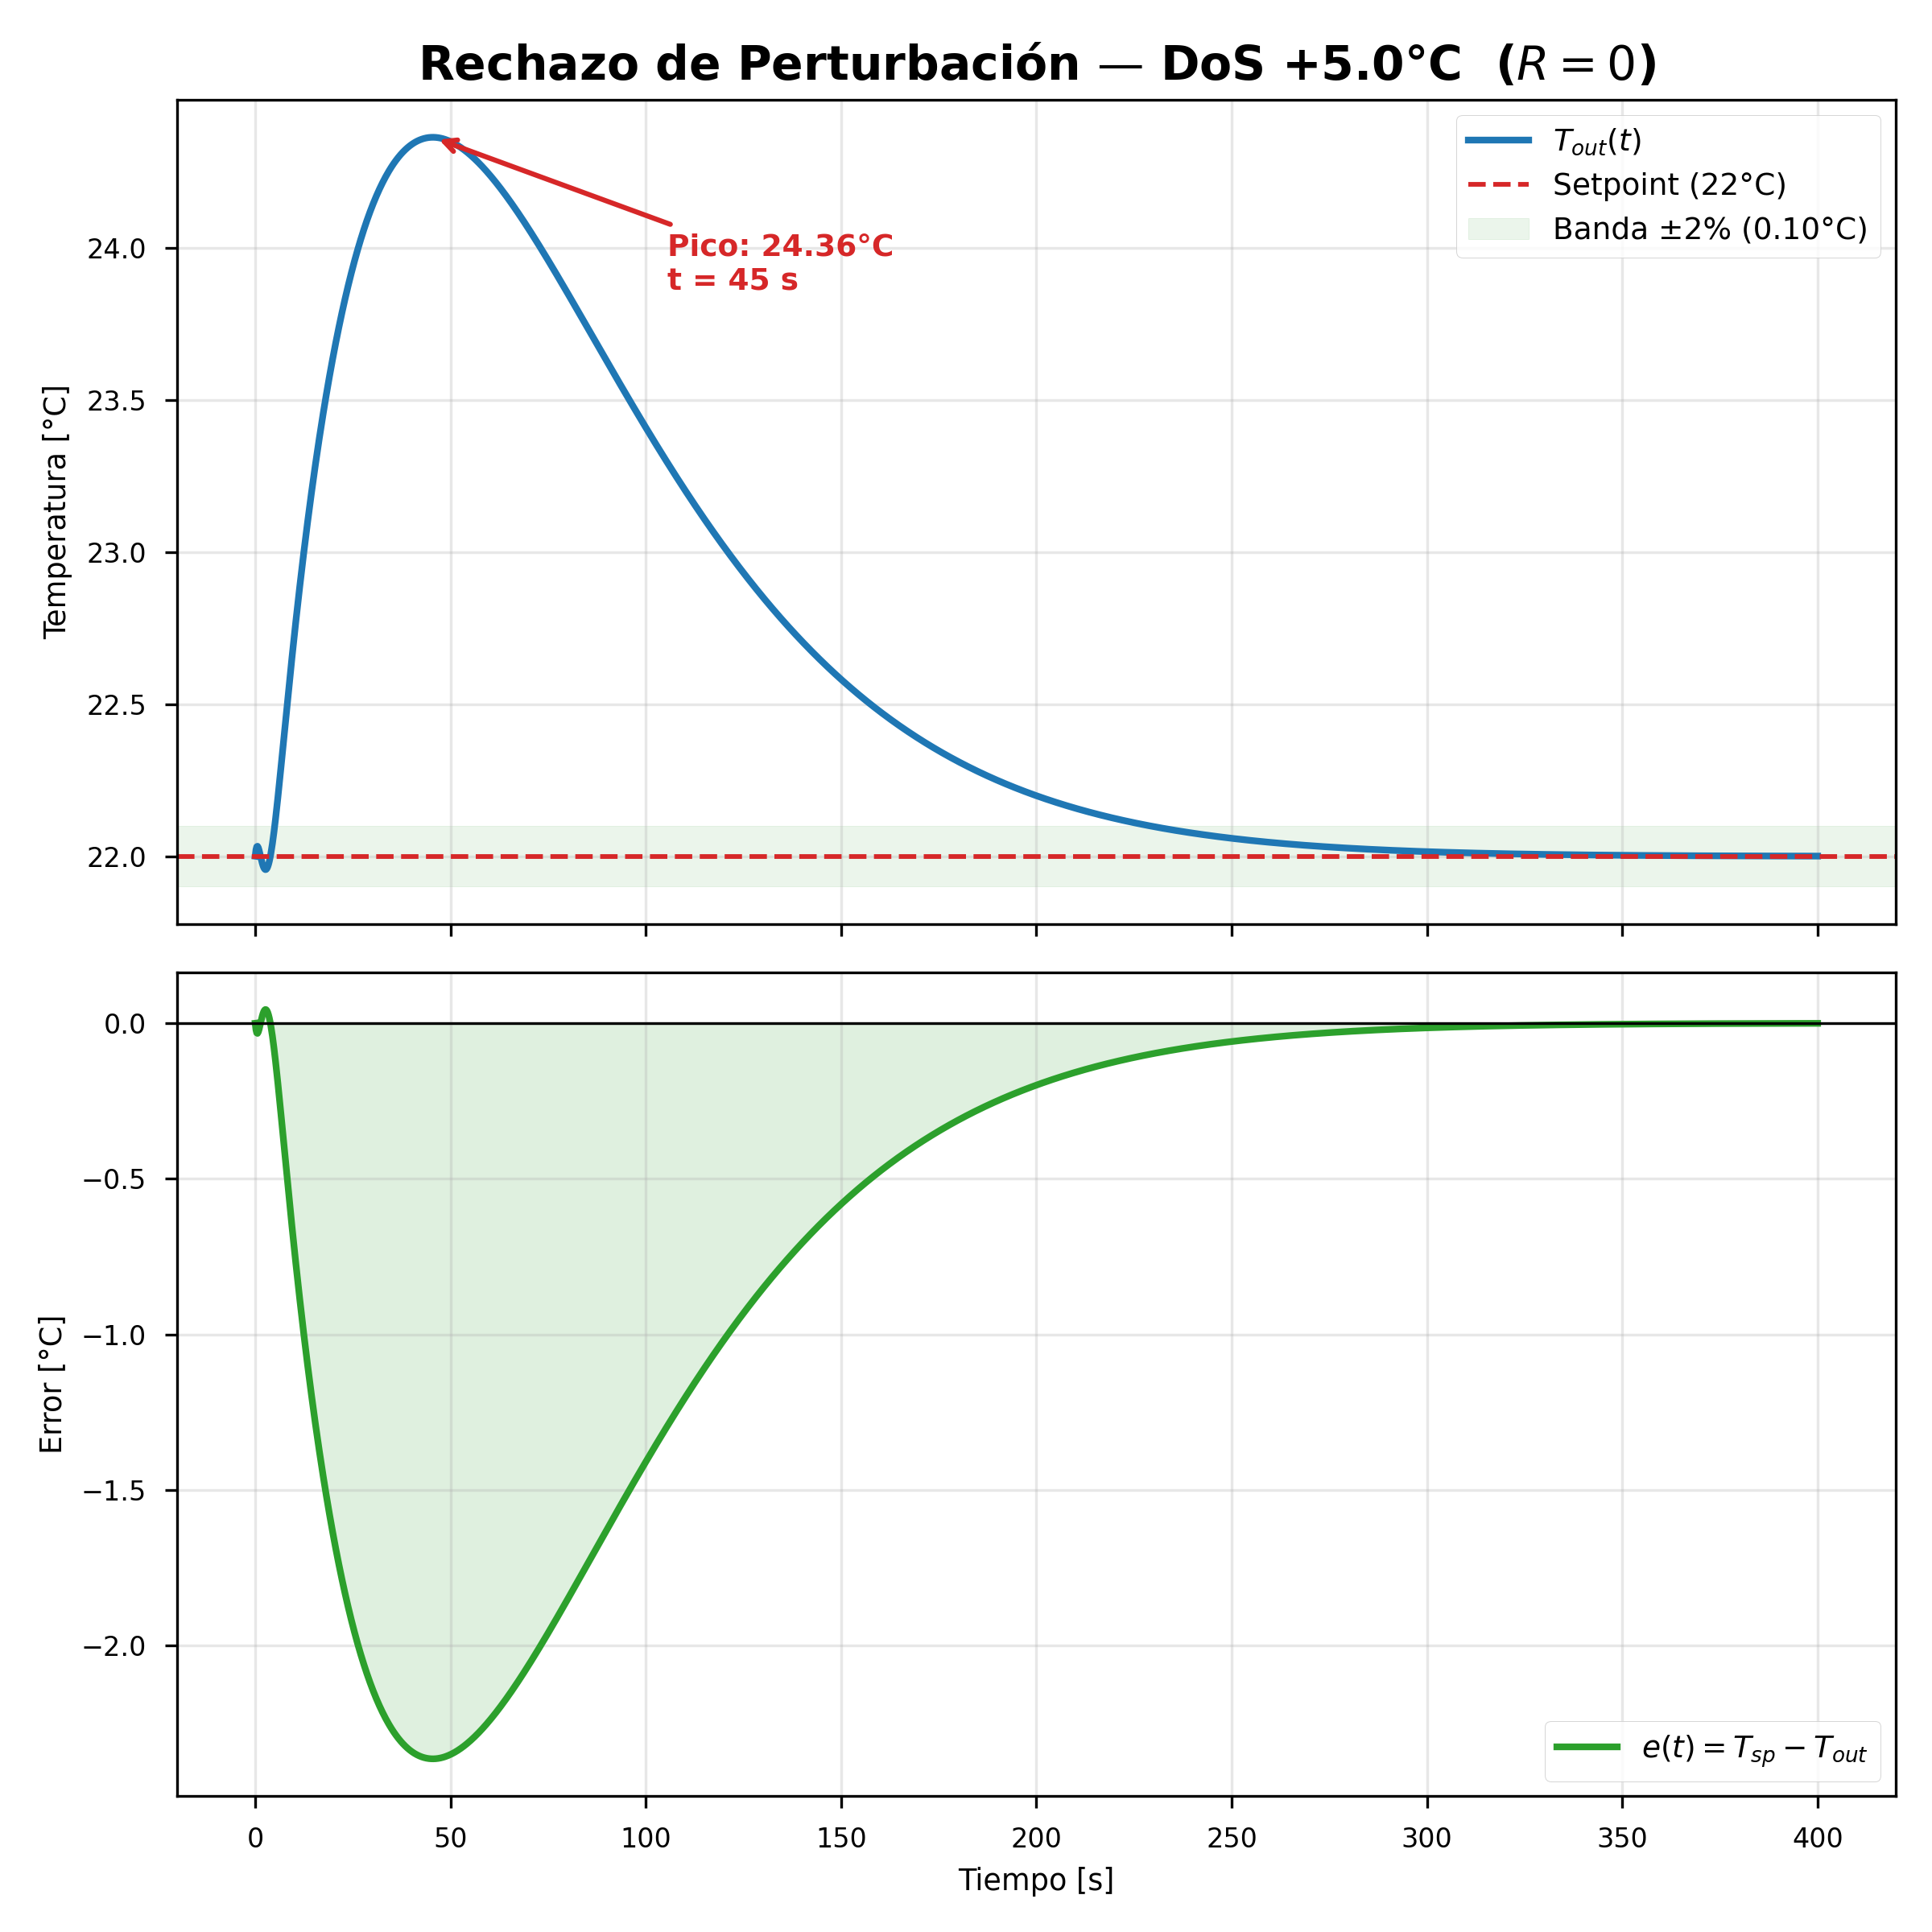
\includegraphics[width=\linewidth]{respuesta_perturbacion.png}
    \caption{Rechazo de perturbación. Partiendo del estado estacionario en $22$\,$^\circ$C, se inyecta un escalón de $+5$\,$^\circ$C filtrado por la dinámica FOPTD del pasillo frío. La temperatura asciende suavemente hasta un pico de $24.36$\,$^\circ$C y es llevada de regreso al setpoint en aproximadamente $229$\,s.}
    \label{fig:perturbacion}
\end{figure}

\subsection{Límites Operativos y Condiciones de Falla}

El actuador CRAC posee una capacidad finita de enfriamiento ($0$-$100$\,\% de apertura). Esta saturación física impone un límite fundamental al rango de perturbaciones que el sistema puede rechazar. Definir este límite es esencial para establecer el dominio de funcionamiento normal y las condiciones bajo las cuales se considera que el sistema falla.

\textbf{Análisis en estado estacionario.} En régimen permanente, la temperatura se estabiliza en el setpoint y el esfuerzo de control debe compensar simultáneamente la diferencia entre la temperatura inicial y la deseada más el efecto de la perturbación. La relación está dada por:
\begin{equation}
    T_{sp} = T_0 + K\,U + D \quad\Longrightarrow\quad U = \frac{T_0 - T_{sp} + D}{|K|}
\end{equation}
Con $K = -0.25$\,\textdegree C/\%, $T_0 = 28$\,\textdegree C y $T_{sp} = 22$\,\textdegree C:
\begin{equation}
    U = 4\,(28 - 22 + D) = 24 + 4D
\end{equation}
El término $24$\,\% corresponde al esfuerzo base necesario para reducir la temperatura desde $28$\,$^\circ$C hasta $22$\,$^\circ$C en ausencia de perturbación.

\textbf{Condición de operación normal.} Para que el sistema mantenga el setpoint sin alcanzar la saturación del actuador se requiere $U \leq 100$\,\%. Sustituyendo:
\begin{equation}
    24 + 4D \leq 100 \quad\Longrightarrow\quad D \leq 19\,^\circ\text{C}
\end{equation}
Para el caso general con una temperatura inicial $T_0$ y un setpoint $T_{sp}$ arbitrarios, el límite es $D \leq 25 - (T_0 - T_{sp})$. Si el sistema ya se encuentra estabilizado en el setpoint al momento de la perturbación ($T_0 \approx T_{sp}$), el límite asciende a $D \leq 25$\,$^\circ$C. La simulación de escritorio permite verificar visualmente este comportamiento: al inyectar un DoS superior al límite, el indicador de estado conmuta a rojo y la temperatura converge a un valor permanentemente alejado del setpoint.

\textbf{Definición de falla por capacidad de refrigeración.} Se considera que el sistema entra en \textbf{falla funcional por capacidad} cuando la perturbación supera el límite calculado y el actuador opera permanentemente saturado, resultando en un error en régimen permanente distinto de cero. Sin embargo, debido a la inercia térmica de la planta, se define un umbral temporal para la detección de la falla: si el esfuerzo de control $u(t)$ permanece saturado al $100\%$ por un tiempo continuo superior a $t_{\text{sat}} \ge 30$\,segundos, se declara el estado de falla del sistema. Esta condición es irreversible sin intervención externa (reducción de la carga térmica o activación de unidades CRAC redundantes).

\textbf{Medidas de mitigación.} En configuraciones típicas de Data Center se emplea redundancia $N+1$: si una unidad CRAC satura, las restantes absorben la carga excedente. Adicionalmente, un lazo de control feedforward que anticipe el aumento de carga térmica a partir de la monitorización del uso de CPU puede iniciar el enfriamiento antes de que la temperatura del aire se eleve, reduciendo el pico transitorio y ampliando el margen efectivo de rechazo.

\subsection{Calidad de Servicio Térmica y Clasificación Dinámica de Estados}

Más allá de la condición de falla por saturación física, el sistema debe cumplir con la normativa **ASHRAE TC 9.9** (Clase A1) para asegurar la integridad de los servidores:
\begin{itemize}
    \item \textbf{Umbral Recomendado ($\le 27$\,$^\circ$C):} Límite térmico óptimo. Superarlo acelera la degradación física del hardware por fatiga térmica.
    \item \textbf{Umbral Límite ($\le 32$\,$^\circ$C):} Límite extremo de operación. Superarlo implica un riesgo inminente de daño físico y activa el apagado automático (\textit{thermal shutdown}) de los equipos.
\end{itemize}

Para evaluar el impacto térmico del ataque DoS durante el transitorio, el simulador calcula en tiempo real tres métricas sencillas de Calidad de Servicio (QoS):
\begin{itemize}
    \item \textbf{Tiempo de Degradación ($t_{>27}$):} Tiempo acumulado (en segundos) en el cual la temperatura del pasillo frío supera los $27$\,$^\circ$C.
    \item \textbf{Tiempo de Falla Térmica ($t_{>32}$):} Tiempo acumulado en el cual la temperatura excede los $32$\,$^\circ$C.
    \item \textbf{Severidad del Desvío (TES):} Representa el área bajo la curva del error térmico (en $^\circ$C$\cdot$s) por encima del setpoint, acumulada desde el inicio del ataque.
\end{itemize}

El simulador de escritorio evalúa dinámicamente las variables físicas de la planta ($T(t)$ y $u(t)$) para clasificar el estado de operación general según la Tabla~\ref{tab:estados}.

\begin{table}[htbp]
\centering
\caption{Criterios de Clasificación Dinámica de Estados}
\label{tab:estados}
\footnotesize
\begin{tabular}{p{1.7cm} p{2.8cm} p{3.2cm}}
\hline
\textbf{Estado} & \textbf{Temperatura} & \textbf{Actuador (CRAC)} \\ \hline
\textbf{Normal (Verde)}  & $T(t) \le 27$\,$^\circ$C & Actuador con margen ($u < 100\%$) \\ \hline
\textbf{Alerta (Amarillo)} & $27 < T(t) \le 32$\,$^\circ$C o bien $T(t) \le 27$\,$^\circ$C & Actuador saturado ($u = 100\%$ por $<30$\,s) pero con consigna segura. \\ \hline
\textbf{Falla (Rojo)}    & $T(t) > 32$\,$^\circ$C o bien $T(t) > 27$\,$^\circ$C & Actuador saturado persistentemente ($u = 100\%$ por $t_{\text{sat}} \ge 30$\,s). \\ \hline
\end{tabular}
\end{table}

\subsection{Análisis del Error en Estado Estable \texorpdfstring{($e_{ss}$)}{e\_ss}}

El sistema de control térmico original posee una realimentación no unitaria debido a la ganancia del sensor de temperatura ($H(s) = 0.2$\,V/$^\circ$C). Dado que las señales en el comparador principal se encuentran en el dominio de tensión eléctrica y no de temperatura, no es posible calcular ni evaluar directamente el error físico de seguimiento como la diferencia de temperatura $R(s) - Y(s)$ desde la señal de error de tensión $E(s)$.

Para calcular de manera rigurosa y conceptual el error en estado estacionario, se aplica el procedimiento clásico de transformación de diagramas de bloques para convertir el lazo original en un lazo equivalente con realimentación unitaria. De este modo, la señal de error se define directamente en la misma unidad física que la variable de consigna ($^\circ$C). En la Fig. \ref{fig:pasos_error} se detallan gráficamente los cuatro pasos de esta transformación.

\begin{figure*}[htbp]
    \centering
    \shorthandoff{<}
    \shorthandoff{>}
    \resizebox{0.95\linewidth}{!}{%
    \begin{tikzpicture}[auto, >=stealth, scale=0.85, transform shape]
        \tikzset{
            block/.style={draw, fill=white, rectangle, minimum height=2.2em, minimum width=5.5em, align=center, line width=0.6pt, rounded corners=1pt, font=\small},
            sum/.style={draw, fill=white, circle, minimum size=1.3em, align=center, line width=0.6pt},
            input/.style={coordinate},
            output/.style={coordinate}
        }
        
        % ---------------------------------------------------------------------
        % (a) DIAGRAMA ORIGINAL
        % ---------------------------------------------------------------------
        \coordinate (orig) at (0,0);
        \node [input] (r_orig) at (orig) {};
        \node [block, right=0.6cm of r_orig] (hr_orig) {$H_r(s) = 0.2$};
        \node [sum, right=0.8cm of hr_orig] (sum_orig) {};
        \node [block, right=0.8cm of sum_orig] (g_orig) {$-G_c(s)G_p(s)$};
        \node [output, right=0.8cm of g_orig] (y_orig) {};
        \node [block, below=0.6cm of g_orig] (h_orig) {$H(s) = 0.2$};
        
        \draw [->, line width=0.6pt] (r_orig) -- node [above, pos=0.15] {$R(s)$} (hr_orig);
        \draw [->, line width=0.6pt] (hr_orig) -- node [above] {$V_{sp}$} (sum_orig);
        \node at ($(sum_orig.center)+(-4pt,4pt)$) {\scriptsize $+$};
        \draw [->, line width=0.6pt] (sum_orig) -- (g_orig);
        \draw [->, line width=0.6pt] (g_orig) -- node [above, pos=0.7] {$Y(s)$} (y_orig);
        \coordinate (split_orig) at ($(g_orig.east)+(0.4,0)$);
        \draw [->, line width=0.6pt] (split_orig) |- (h_orig.east);
        \draw [->, line width=0.6pt] (h_orig.west) -| (sum_orig.south);
        \node at ($(sum_orig.center)+(-4pt,-4pt)$) {\scriptsize $-$};
        
        \node at ($(orig) + (3.5, -2.5)$) [font=\bfseries] {(a) Lazo original con realimentación no unitaria ($H_r, H \neq 1$)};

        % ---------------------------------------------------------------------
        % (b) REORGANIZACIÓN (ABSORBER Hr)
        % ---------------------------------------------------------------------
        \coordinate (step1) at (9.5,0);
        \node [input] (r_s1) at (step1) {};
        \node [sum, right=0.6cm of r_s1] (sum_s1) {};
        \node [block, right=0.8cm of sum_s1, minimum width=8.5em] (g_s1) {$G'(s) = -H_r(s)G_c(s)G_p(s)$};
        \node [output, right=1.2cm of g_s1] (y_s1) {};
        \node [block, below=0.6cm of g_s1] (h_s1) {$H'(s) = \frac{H(s)}{H_r(s)}$};
        
        \draw [->, line width=0.6pt] (r_s1) -- node [above, pos=0.15] {$R(s)$} (sum_s1);
        \node at ($(sum_s1.center)+(-4pt,4pt)$) {\scriptsize $+$};
        \draw [->, line width=0.6pt] (sum_s1) -- (g_s1);
        \draw [->, line width=0.6pt] (g_s1) -- node [above, pos=0.9] {$Y(s)$} (y_s1);
        \coordinate (split_s1) at ($(g_s1.east)+(0.6,0)$);
        \draw [->, line width=0.6pt] (split_s1) |- (h_s1.east);
        \draw [->, line width=0.6pt] (h_s1.west) -| (sum_s1.south);
        \node at ($(sum_s1.center)+(-4pt,-4pt)$) {\scriptsize $-$};
        
        \node at ($(step1) + (3.5, -2.5)$) [font=\bfseries] {(b) Reorganización con entrada directa $R(s)$ ($H'(s) = H/H_r$)};

        % ---------------------------------------------------------------------
        % (c) DIVISIÓN EN CASCADA (REALIMENTACIÓN INTERNA)
        % ---------------------------------------------------------------------
        \coordinate (step2) at (0,-4.5);
        \node [input] (r_s2) at (step2) {};
        \node [sum, right=0.8cm of r_s2] (sum_s2a) {};
        \node [sum, right=1.2cm of sum_s2a] (sum_s2b) {};
        \node [block, right=1.2cm of sum_s2b] (g_s2) {$G'(s)$};
        \node [output, right=1.8cm of g_s2] (y_s2) {};
        \node [block, below=0.7cm of g_s2] (h_s2) {$H'(s) - 1$};
        
        \draw [->, line width=0.6pt] (r_s2) -- node [above, pos=0.15] {$R(s)$} (sum_s2a);
        \node at ($(sum_s2a.center)+(-4pt,4pt)$) {\scriptsize $+$};
        \draw [->, line width=0.6pt] (sum_s2a) -- node [above] {$\varepsilon(s)$} (sum_s2b);
        \node at ($(sum_s2b.center)+(-4pt,4pt)$) {\scriptsize $+$};
        \draw [->, line width=0.6pt] (sum_s2b) -- node [above] {$E_a(s)$} (g_s2);
        \draw [->, line width=0.6pt] (g_s2) -- node [above, pos=0.85] {$Y(s)$} (y_s2);
        
        \coordinate (split_s2) at ($(g_s2.east)+(0.8,0)$);
        % Realimentación unitaria (Línea verde)
        \draw [->, line width=0.6pt, green!60!black] (split_s2) |- ++(0,-2.5) -| (sum_s2a.south);
        \node at ($(sum_s2a.center)+(-4pt,-4pt)$) {\scriptsize $-$};
        
        % Realimentación auxiliar H'-1
        \draw [->, line width=0.6pt] ($(split_s2)+(0,-0.3)$) |- (h_s2.east);
        \draw [->, line width=0.6pt] (h_s2.west) -| (sum_s2b.south);
        \node at ($(sum_s2b.center)+(-4pt,-4pt)$) {\scriptsize $-$};
        
        \node at ($(step2) + (3.5, -3.5)$) [font=\bfseries] {(c) Separación en cascada de la realimentación unitaria};

        % ---------------------------------------------------------------------
        % (d) LAZO UNITARIO SIMPLIFICADO
        % ---------------------------------------------------------------------
        \coordinate (step3) at (9.5,-4.5);
        \node [input] (r_s3) at (step3) {};
        \node [sum, right=0.8cm of r_s3] (sum_s3) {};
        \node [block, right=1.2cm of sum_s3, minimum width=9.5em] (g_s3) {$G_e(s) = \frac{G'(s)}{1 + G'(s)(H'(s)-1)}$};
        \node [output, right=1.8cm of g_s3] (y_s3) {};
        
        \draw [->, line width=0.6pt] (r_s3) -- node [above, pos=0.15] {$R(s)$} (sum_s3);
        \node at ($(sum_s3.center)+(-4pt,4pt)$) {\scriptsize $+$};
        \draw [->, line width=0.6pt] (sum_s3) -- node [above, pos=0.5] {$\varepsilon(s)$} (g_s3);
        \draw [->, line width=0.6pt] (g_s3) -- node [above, pos=0.9] {$Y(s)$} (y_s3);
        
        \coordinate (split_s3) at ($(g_s3.east)+(0.8,0)$);
        \draw [->, line width=0.6pt] (split_s3) |- ++(0,-1.5) -| (sum_s3.south);
        \node at ($(sum_s3.center)+(-4pt,-4pt)$) {\scriptsize $-$};
        
        \node at ($(step3) + (3.5, -3.5)$) [font=\bfseries] {(d) Lazo unitario simplificado equivalente};
        
    \end{tikzpicture}%
    }
    \shorthandon{<}
    \shorthandon{>}
    \caption{Procedimiento paso a paso para la transformación de un lazo con realimentación no unitaria en un lazo equivalente de realimentación unitaria, exponiendo directamente el error de seguimiento físico $\varepsilon(s) = R(s) - Y(s)$ en la misma unidad física de la referencia ($^\circ$C).}
    \label{fig:pasos_error}
\end{figure*}

El desglose físico-matemático de cada etapa del procedimiento es el siguiente:

\textbf{1. Paso (a) a Paso (b): Reorganización y desplazamiento de bloques.}
El lazo cerrado original cumple con la relación de salida:
\begin{equation}
    Y(s) = \frac{-G_c(s)G_p(s)H_r(s)}{1 - G_c(s)G_p(s)H(s)} \cdot R(s)
\end{equation}
Para colocar a la referencia física $R(s)$ en el comparador de entrada, desplazamos la ganancia $H_r(s)$ pasándola al interior del lazo, lo que equivale a multiplicar la trayectoria directa original por $H_r(s)$ y a dividir el lazo de realimentación por el mismo factor. Esto define un bloque directo equivalente $G'(s)$ y una realimentación equivalente $H'(s)$:
\begin{align}
    G'(s) &= -H_r(s) G_c(s) G_p(s) \\
    H'(s) &= \frac{H(s)}{H_r(s)}
\end{align}
Esta configuración (Paso b) conserva de forma exacta la transferencia de lazo cerrado, permitiendo realizar comparaciones térmicas en el nodo sumador de entrada.

\textbf{2. Paso (b) a Paso (c): Suma y resta de realimentación unitaria.}
En un lazo no unitario, la realimentación hacia el comparador es $Y(s)H'(s)$, lo que genera un error que no equivale al desvío real $R(s) - Y(s)$. Para obtener la señal del error de seguimiento físico $\varepsilon(s) = R(s) - Y(s)$, sumamos y restamos un camino de realimentación unitaria en paralelo. La señal de realimentación modificada se descompone como:
\begin{equation}
    Y(s)H'(s) = Y(s) \cdot 1 + Y(s)(H'(s) - 1)
\end{equation}
Esto nos permite bifurcar la señal en dos comparadores en cascada (Paso c): el comparador externo calcula el error físico de seguimiento $\varepsilon(s) = R(s) - Y(s)$, y el comparador interno procesa el término de ajuste $Y(s)(H'(s)-1)$.

\textbf{3. Paso (c) a Paso (d): Simplificación del lazo interno.}
El lazo de realimentación secundario interno tiene como bloque de trayectoria directa a $G'(s)$ y como bloque de realimentación a $H'(s)-1$. La transferencia reducida de este sub-lazo genera la trayectoria directa equivalente $G_e(s)$ del lazo unitario final:
\begin{equation}
    G_e(s) = \frac{G'(s)}{1 + G'(s)(H'(s) - 1)}
\end{equation}
El sistema se reduce así a un lazo unitario equivalente (Paso d), donde la relación entre el error de seguimiento $\varepsilon(s)$ y la referencia es:
\begin{equation}
    \varepsilon(s) = R(s) - Y(s) = \frac{R(s)}{1 + G_e(s)}
\end{equation}

\textbf{Aplicación al sistema con instrumentación simétrica.}
Dado que el transmisor de referencia y el sensor de realimentación poseen la misma ganancia ($H_r(s) = H(s) = 0.2$\,V/$^\circ$C), el factor de realimentación equivalente es unitario y el término de realimentación interna secundaria se anula:
\begin{align}
    H'(s) &= \frac{0.2}{0.2} = 1 \\
    H'(s) - 1 &= 0
\end{align}
Esto simplifica de forma inmediata la trayectoria directa equivalente a:
\begin{equation}
    G_e(s) = G'(s) = -0.2\,G_c(s)G_p(s)
\end{equation}

Utilizando la función de transferencia del lazo unitario equivalente, aplicamos el Teorema del Valor Final para analizar analíticamente el error en régimen permanente.

\textbf{1. Error de seguimiento ante escalón de referencia.}
Para un cambio tipo escalón en la temperatura deseada de magnitud $T$, la entrada es $R(s) = T/s$. El error en estado estacionario se calcula como:
\begin{equation}
    e_{ss} = \lim_{s \to 0} s \cdot \varepsilon(s) = \lim_{s \to 0} \frac{s \cdot (T/s)}{1 + G_e(s)} = \lim_{s \to 0} \frac{T}{1 + G_e(s)}
\end{equation}
El controlador PID paralelo incluye una acción integral con ganancia $K_i/s$. Al evaluar el límite en baja frecuencia ($s \to 0$), la transferencia del controlador tiende a infinito ($G_c(0) \to \infty$), lo que a su vez causa que la trayectoria equivalente tienda a infinito ($G_e(0) \to \infty$). Al evaluar el límite del error permanente:
\begin{equation}
    e_{ss} = \lim_{s \to 0} \frac{T}{1 + G_e(s)} = 0
\end{equation}
Este resultado analítico garantiza un error de seguimiento nulo ante cambios sostenidos en el setpoint térmico.

\textbf{2. Error de seguimiento ante escalón de perturbación.}
Con la entrada de consigna anulada ($R(s) = 0$), el error físico es $\varepsilon(s) = -Y(s)$. A partir de la transferencia de lazo cerrado ante perturbaciones obtenida en la Sección V-B, la salida $Y(s)$ en función de la trayectoria equivalente del lazo unitario $G_e(s)$ se expresa como:
\begin{equation}
    \frac{Y(s)}{D(s)} = \frac{1}{1 - G_c(s)G_p(s)H(s)} = \frac{1}{1 + G_e(s)}
\end{equation}
Por lo tanto, la señal de error ante perturbaciones térmicas es:
\begin{equation}
    \varepsilon(s) = -Y(s) = -\frac{D(s)}{1 + G_e(s)}
\end{equation}
Para la perturbación térmica real asociada al ataque DoS, cuya dinámica se modela filtrada por la inercia de la planta y el retardo, la transformada de Laplace es:
\begin{equation}
    D(s) = \frac{d \cdot e^{-4.5 s}}{s \cdot (35 s + 1)}
\end{equation}
donde $d$ representa la magnitud del salto térmico de la perturbación. Calculamos el error permanente en estado estable aplicando el Teorema del Valor Final:
\begin{align}
    e_{ss} &= \lim_{s \to 0} s \cdot \varepsilon(s) \nonumber \\
           &= \lim_{s \to 0} s \cdot \left[ - \frac{d \cdot e^{-4.5 s}}{s \cdot (35 s + 1)} \cdot \frac{1}{1 + G_e(s)} \right] \nonumber \\
           &= \lim_{s \to 0} - \frac{d \cdot e^{-4.5 s}}{(35 s + 1)(1 + G_e(s))}
\end{align}
Al evaluar el límite cuando $s \to 0$:
- La inercia térmica tiende a la unidad: $35 s + 1 \to 1$.
- El término de retardo tiende a la unidad: $e^{-4.5 s} \to 1$.
- La trayectoria directa equivalente tiende a infinito debido al integrador: $G_e(0) \to \infty$.
Sustituyendo estos límites, se demuestra de forma rigurosa que el error en estado estable es nulo:
\begin{equation}
    e_{ss} = -\frac{d \cdot 1}{1 \cdot (1 + \infty)} = 0
\end{equation}
La presencia de la acción integral asegura este rechazo completo de la perturbación térmica sostenida, retornando la temperatura del pasillo frío al valor del setpoint seleccionado sin desvío permanente.

\textbf{Conclusión.} Tanto en el seguimiento de referencia como en el rechazo de perturbaciones, el error en régimen permanente es nulo. La acción integral es el único término del controlador que garantiza este resultado: sin el integrador ($K_i = 0$), $G_e(0)$ sería finito y existiría un error remanente proporcional a la magnitud de la excitación, inaceptable en un entorno donde la estabilidad térmica es crítica para la integridad del equipamiento de TI.


\subsection{Superposición de Respuestas}

\begin{figure}[htbp]
    \centering
    
\includegraphics[width=\linewidth]{respuesta_temporal.png}
    \caption{Respuesta completa del sistema. Superposición del seguimiento al escalón de referencia ($28 \to 22$\,$^\circ$C) y el rechazo del ataque DoS inyectado en $t = 200$\,s. En ambas fases el error en régimen permanente es nulo.}
    \label{fig:temporal}
\end{figure}

La Fig.~\ref{fig:temporal} reúne visualmente los dos fenómenos analizados en las secciones anteriores. La curva graficada es la superposición de la respuesta al escalón de referencia (Sección V-A) y la respuesta al ataque DoS (Sección V-B). En el dominio de Laplace, para $0 \leq t < 200$\,s la temperatura evoluciona según:
\begin{equation}
    Y_{track}(s) = \frac{28}{s} + \frac{-0.2\,G_c(s)\,G_p(s)}{1 - 0.2\,G_c(s)\,G_p(s)} \cdot \frac{-6}{s}
\end{equation}
y para $t \geq 200$\,s se superpone la contribución de la perturbación:
\begin{equation}
    Y(s) = Y_{track}(s) + \frac{1}{1 - G_c(s)\,G_p(s)\,H(s)} \cdot \frac{5 \cdot e^{-4.5 s}}{s \cdot (35 s + 1)}
\end{equation}
Se observa que en ambos tramos el error converge a cero, confirmando analítica y experimentalmente la eficacia de la acción integral.
\FloatBarrier
\section{Conclusión}
En este trabajo final integrador, se ha diseñado, modelado y validado con éxito un sistema de control clásico en lazo cerrado para la regulación de la temperatura en el pasillo frío de un Data Center, garantizando el cumplimiento de los estrictos rangos operativos definidos por la normativa ASHRAE TC 9.9 y tomando como base el modelo fluidodinámico de Shi et al. (2026). 

A partir del desarrollo realizado, se destacan las siguientes conclusiones de carácter ingenieril:
\begin{itemize}
    \item \textbf{Rol Crítico de la Acción Integral:} Mediante la transformación formal del lazo de realimentación no unitaria a un lazo equivalente de realimentación unitaria y la aplicación del Teorema del Valor Final, se demostró analíticamente que la acción integral ($K_i$) del controlador PID paralelo es el único término capaz de garantizar un error de seguimiento físico en estado estable nulo ($e_{ss} = 0$). Este resultado se cumple tanto ante escalones de referencia de temperatura como frente a la perturbación de calentamiento del ataque DoS de $+5^\circ$C. Sin esta acción integral, el sistema presentaría un desvío permanente (*offset*) inaceptable para la integridad térmica del hardware de TI.
    \item \textbf{Validación Multi-Entorno:} La correspondencia exacta entre la simulación continua en tiempo real desarrollada en Python/Streamlit y el modelado discreto por bloques en Scilab/Xcos permitió validar experimentalmente el diseño. Este enfoque híbrido posibilitó ensayar el comportamiento del controlador incorporando no linealidades reales del sistema físico, tales como la saturación de los ventiladores EC de la CRAC ($0-100\%$) y la escala analógica del transductor de temperatura ($H = 0.2$\,V/$^\circ$C).
    \item \textbf{Eficiencia Energética y Control Feedforward:} Para mitigar el pico térmico transitorio de $24.37^\circ$C provocado por el ataque DoS, se propuso la incorporación de un control Feedforward (Prealimentación). Dado que la disipación térmica es directamente proporcional a la carga de CPU de los servidores (la cual puede medirse instantáneamente a nivel de software), esta señal se puede inyectar al lazo de control de forma predictiva. Esto permite a la CRAC iniciar el enfriamiento del pasillo antes de que el aire caliente alcance al sensor Pt100, eludiendo el retardo de transporte y mejorando la eficiencia energética global del sistema al evitar el sobre-enfriamiento.
\end{itemize}

En síntesis, este trabajo demuestra que la aplicación rigurosa de la Teoría de Control clásica constituye una herramienta indispensable en el diseño de infraestructuras tecnológicas modernas, logrando un balance óptimo entre la seguridad operativa de los equipos electrónicos y la optimización de los recursos energéticos.

\begin{thebibliography}{5}
\bibitem{liu2026} Shi, H., Pan, S., Liu, K., Wan, T., Li, C., \& Niu, B. (2026). \textit{Optimizing Control Chain Latency in Liquid Cooled Data Center for Load Responsive Operation}. Buildings, MDPI, 16(9), 1752. DOI: 10.3390/buildings16091752.
\bibitem{ashrae} ASHRAE TC 9.9 (2021). \textit{Thermal Guidelines for Data Processing Environments}.
\bibitem{parolini} Parolini, L., et al. (2012). \textit{A Cyber-Physical Systems Approach to Data Center Modeling and Control}. Proceedings of the IEEE.
\bibitem{ogata} Ogata, K. (2010). \textit{Ingeniería de Control Moderna}. Pearson.
\bibitem{schneider} Schneider Electric (2023). \textit{Technical Specifications: Uniflair™ Direct Expansion Room Cooling Solutions}. White Paper.
\end{thebibliography}

\clearpage
\onecolumn
\appendix
\section{Apéndice: Pautas Reglamentarias del Trabajo Final Integrador}
A continuación, se reproduce la copia fiel del documento de pautas provisto por la cátedra para el desarrollo del Trabajo de Integración, de cumplimiento formal requerido para la entrega del informe final.

\begin{lstlisting}[basicstyle=\ttfamily\scriptsize, frame=single, breaklines=true, numbers=left, stepnumber=1]
Pautas para el desarrollo del Trabajo Final de Tecnologias de Automatizacion

    1. Objeto de este documento

Proporcionar una guia de orientacion para el desarrollo del Trabajo de Integracion de la materia, en lo concerniente al bloque tematico de la Teoria de Control (oportunamente explicitado en sucesivas clases desde el inicio de la cursada).
Contiene el proposito, objetivos del trabajo, las pautas a seguir y las recomendaciones correspondientes.

    2. Proposito

    * Aplicar la totalidad de los conceptos fundamentales de la Teoria de Control a un sistema elegido por cada equipo de trabajo.

    3. Objetivos Generales

    * Seleccionar un sistema de control aplicado a una solucion tecnologica (preferentemente, del area de Sistemas de la Informacion). Es importante destacar que el sistema elegido debera existir en el mercado, siendo utilizado a modo de modelo de analisis. 

    * Fundamentar el sistema propuesto utilizando, a modo de marco teorico, los conceptos, fundamentos, enfoques y estrategias de la Ingenieria de Control.

    * Aplicar diferentes tecnicas o herramientas informaticas, en forma creativa, para realizar graficos, modelos, cuadros comparativos, y, en general para expresar el analisis del problema y la solucion propuesta.

    * Basar el desarrollo del trabajo en el analisis y criterio individual de los integrantes del equipo, de manera tal de elaborar una produccion propia basada en los aspectos descriptivo, funcionales y prospectivo del sistema en cuestion. 

    4. Pautas

    * Desarrollo del trabajo

El trabajo de investigacion sera desarrollado por equipos de no mas de dos integrantes.
La fecha de entrega del Trabajo Final sera informada mediante la plataforma del webcampus. Esta fecha permitira la correccion del mismo antes de la primera fecha de llamado a final.

Para el caso de que el TP no sea aprobado y requiera de correcciones y/o mayor desarrollo, o no haya sido presentado hasta la fecha indicada, se estipulara una nueva fecha tope de entrega mediante el mismo procedimiento.

Una vez aprobado el TP, y en caso de tener cumplimentadas la totalidad de las actividades obligatorias pautadas, el alumno estara en condiciones de firmar la materia.

La entrega se realizara en formato de archivo PDF por cada alumno en el web campus del curso (en el sitio dedicado a tal efecto). 
En cada trabajo se incluira en la caratula el listado de integrantes del grupo.
Pueden realizarse consultas durante el periodo de desarrollo.

    *  Composicion del Trabajo de Investigacion 

El trabajo, desde el punto de vista formal, estara compuesto de las siguientes partes:

    * Caratula: incluye el titulo del tema, nombre y apellido de los integrantes del equipo de trabajo, la comision, el nombre y apelido del profesor, la fecha de entrega.

    * Copia del presente documento.

    * Indice: contenido del documento elaborado por el equipo.

    * Introduccion: se referira al "segmento / mercado" en que se encuadra el trabajo (por ejemplo, "...el control del riego y la fertilizacion de una plantacion...").

    * Objetivos: cuales son los objetivos de control a ser alcanzados y cual es la solucion que se plantea u ofrece.

    * Alcance: definir la estructura del sistema considerado, describiendo e identificando clara y explicitamente las diferentes funcionalidades correspondientes al mismo (por ejemplo: contexto; tipo de carga a considerar; puntos de interconexion con el mundo exterior; tipos de transductores; variables que se desea controlar, tipos de unidades y rangos de entradas y salidas, amplificador de error; senales de error y realimentacion; elementos de medicion, caracteristicas y variables componentes de las transferencias presentes en el sistema ; caracteristicas de la respuesta; perturbaciones externas e internas a considerar; caracteristicas y tipo de error; caracterizacion de la estabilidad; ley de control y tipo de actuacion utilizada; relacion entre senales analogicas y discretas / digitales; carga/s asociadas al sistema).

El trabajo debera incluir un programa confeccionado en lenguaje de alto nivel a eleccion, que permita simular y verificar en tiempo real la funcionalidad del sistema mediante la interrelacion de las senales / variables del mismo.

IMPORTANTE: Tal lo explicitado en clase, no se solicita la descripcion generica del sistema controlado sino la identificacion y descripcion de su estructura.

En definitiva, "encontrar" la totalidad de los contenidos y conceptos trabajados y estudiados desde el dominio de la teoria de control.

    * Descripcion, desarrollo y fundamentacion de la propuesta: debe ser clara, recomendandose tecnicas de escritura conceptual y grafica.	

    * Conclusion: A modo de conclusion, establecer la necesidad y ventajas comparativas del sistema de control propuesto. Es importante incluir opiniones propias en cuanto a posibles mejoramientos, limitaciones analiticas, etc., que permitan establecer un cierto criterio ingenieril desde la perspectiva del equipo de trabajo.

    * Consideraciones especiales: si aplica, indicar.

    * Bibliografia: citar libros, documentos de texto y fotograficos, folletos de dispositivos transductores, actuadores, sitios web y papers consultados.

                                Drando. Omar Civale
\end{lstlisting}

\end{document}
